\documentclass[a4paper,10pt]{report}
\usepackage[utf8]{inputenc}
\usepackage{cancel}
\usepackage[margin=2cm]{geometry}
\usepackage{amsmath}
\usepackage{amssymb}
\usepackage{undertilde}
\usepackage{graphicx}
\usepackage{hyperref}
\usepackage{gensymb}

% user defined commands
\newcommand{\Comb}[2]{{}^{#1}C_{#2}}
\newcommand{\note}[1]{\begin{center}\emph{NOTE: {#1}}\end{center}}

% user defined environments
\newenvironment{example}{For example:\\}{}

% Change abstract name
\renewcommand{\abstractname}{The pourpose}

\graphicspath{ {./images} }

% Title Page
\title{Mathematical Specialists}
\author{Lachlan Takumi Ikeguchi}

\begin{document}
\maketitle
\tableofcontents

\begin{abstract}
	This document was written to be used as a summary to help revise the content covered mathematical specialists.  For any inquiries, feedback, and further explanations, contact lachlanprivate@duck.com or through the discord server: https://discord.gg/6P8rddkXFr .  I encourage you to let me know of any topic I missed, how I could explain it better, or how it could be reworded or formatted to be more helpful in it's purpose.  The goal of this document is to be a comprehensive summary of everything you need to know.
\end{abstract}

\section{Important symbols}
\begin{center}
	\begin{tabular}{l|lp{6cm}}
		Symbol         & Mathematical definition                                                  & Simple definition                                                                                              \\ \hline
		$\cup$         & Union                                                                    & $A$ \emph{and} $B$, or think as in 'add'.                                                                      \\
		$\cap$         & Intersection                                                             & $A$ \emph{or} $B$, or think as in 'multiply'.                                                                  \\
		$n!$           & $n \times (n-1) \times (n-2) \times (n-3)... \times 3 \times 2 \times 1$ & The product of integers between the given value and 1.                                                         \\
		$^nP_r$        & $\frac{n!}{(n-r)!}$                                                      & The number of combinations there are of length $r$ from a group of length $n$ where the order matters.         \\
		$^nC_r$        & $\frac{\frac{n!}{(n-r)!}}{r!}$ or $\frac{n!}{r!(n - r)!}$                & The number of combinations there are of length $r$ from a group of length $n$ where the order does not matter. \\
		$\binom{n}{r}$ & $^nC_r$                                                                  & The same as the combinations but in a different notation.
	\end{tabular}
\end{center}

\pagebreak

\section{Addition principle}
If there are $n$ ways of performing operation $A$, and $m$ ways of performing operation $B$, there are $n + m$ ways of performing operation $A \cap B$.\\

As in, let there be 2 ways to perform task $A$, and 3 ways to perform task $B$.  If there is an option to perform $A$ \emph{or} $B$, there is a total of $2 + 3 = 5$ ways to perform an operation.


\section{Multiplication principle}
If there are $n$ ways of performing operation $A$, and $m$ ways of performing operation $B$, there are $n \times m$ ways of performing operation $A \cup B$.\\

As in, let there be 4 ways to perform task $A$, and 5 ways to perform task $B$.  With considering 1 way to perform $A$, there are 5 ways to perform $B$, repeat the process through the number of ways to perform $A$.
\begin{center}
	\begin{tabular}{l|lllll}
		       & $B$, 1 & $B$, 2 & $B$, 3 & $B$, 4 & $B$, 5 \\ \hline
		$A$, 1 & (1, 1) & (1, 2) & (1, 3) & (1, 4) & (1, 5) \\
		$A$, 2 & (2, 1) & (2, 2) & (2, 3) & (2, 4) & (2, 5) \\
		$A$, 3 & (3, 1) & (3, 2) & (3, 3) & (3, 4) & (3, 5) \\
		$A$, 4 & (4, 1) & (4, 2) & (4, 3) & (4, 4) & (4, 5) \\
	\end{tabular}
\end{center}
Where there are $4 \times 5 = 20$ ways to perform the operations.


\section{Factorials}
Factorials is the result of multiplying all of the integers between the given integer and 1.  This is given the notation and formula:
$$
	n! = n \times (n-1) \times (n-2) \times (n-3)... \times 3 \times 2 \times 1
$$
Example:\\
\begin{align*}
	5! & = 5 \times 4 \times 3 \times 2 \times 1 \\
	   & = 120
\end{align*}


\subsection{Dividing factorials}
When given some factorial over another factorial in such cases as:
$$\frac{4!}{2!}$$
$$\frac{4 \times 3 \times 2 \times 1}{2 \times 1}$$
$$\frac{4 \times 3 \times \cancel{2 \times 1}}{\cancel{2 \times 1}}$$
$$4 \times 3$$
$$12$$

\subsection{Special cases}
$$0! = 1$$

\section{Permutations}
Permutations is the number of ways of choosing $r$ things from $n$ distinct things where \emph{order matters}.  This is given the notation and formula:
$$
	^nP_r = \frac{n!}{(n-r)!}
$$
Example:\\
\begin{align*}
	^6P_4 & = \frac{6!}{(6 - 4)!}                                                                 \\
	      & = \frac{6!}{2!}                                                                       \\
	      & = \frac{6 \times 5 \times 4 \times 3 \times 2 \times 1}{2 \times 1}                   \\
	      & = \frac{6 \times 5 \times 4 \times 3 \times \cancel{2 \times 1}}{\cancel{2 \times 1}} \\
	      & = 6 \times 5 \times 4 \times 3                                                        \\
	      & = 360
\end{align*}

\subsection{Permutations in a circle}
In cases where the positions being concerned is a circle such as the permutations of a circular seating arrangement, if the standard permutations formula is applied, there are several over-counting of the like arrangement in a different perspective.  In these cases apply the formula:
$$
	\frac{^nP_r}{r} = \frac{\frac{n!}{(n-r)!}}{r}
$$

\subsection{Like objects repetitions}
The number of ways of arranging $n$ objects made up of indistinguishable objects, $n_1$ in the first group, $n_2$ in the second group and so on, is:
$$
	\frac{n!}{n_1! n_2! n_3!... n_r!}
$$
Example:\\
\begin{center}
	Find the number of permutations of the letters in the world WOOLLOOMOOLOO.\\
	There are 8 'O's and 3 'L's\\
	Permutations:
	$$\frac{13!}{8!3!}$$
	$$\frac{13 \times 12 \times 11 \times 10 \times 9 \times 8 \times 7 \times 6 \times 5 \times 4 \times 3 \times 2 \times 1}{(8 \times 7 \times 6 \times 5 \times 4 \times 3 \times 2 \times 1) \times (3 \times 2 \times 1)}$$
	$$\frac{13 \times 12 \times 11 \times 10 \times 9 \cancel{\times 8 \times 7 \times 6 \times 5 \times 4 \times 3 \times 2 \times 1}}{\cancel{(8 \times 7 \times 6 \times 5 \times 4 \times 3 \times 2 \times 1)} \times (3 \times 2 \times 1)}$$
	$$\frac{13 \times 12 \times 11 \times 10 \times 9}{3 \times 2}$$
	$$\frac{13 \times \cancelto{6 \cancel{\times 2}}{12} \times 11 \times 10 \times \cancelto{3 \cancel{\times 3}}{9}}{\cancel{3 \times 2}}$$
	$$13 \times 6 \times 11 \times 10 \times 3$$
	$$25,740$$
\end{center}

\subsection{Restrictions}
When considering restrictions, deal with the restrictions first.\\
Example:\\
\begin{center}
	Find the number of arrangements of the letters of the word DARWIN beginning and ending with a vowel.\\
	Number of letters = 6\\
	Number of positions = 6\\
	Beginning and end must be a vowel, so the available positions are decreased by 2: number of positions - 2 = 4\\
	Since 2 vowels must be used:  number of letters - 2 = 4\\
	Permutations:
	$$^4P_4$$
	$$4!$$
	$$4 \times 3 \times 2 \times 1$$
	$$24$$
\end{center}

\subsection{Grouped items}
When items are grouped together, treat each group as a single object.  Find the number of arrangements of the groups, then multiply by the number of arrangement within each group.\\
Example:\\
\begin{center}
	Find the number of arrangement of the letters of the word EQUALS if the vowels are kept together.\\
	Number of vowels = 3\\
	Number of letters = 6\\
	Number of positions = 6\\
	As the 3 vowels are grouped together, the number of positions decreases:\\ number of positions - 3\textsubscript{for the members of the group} + 1\textsubscript{for the group} = 4\\
	Permutations within vowel group:
	$$^3P_3 = 3! = 3 \times 2 = 6$$
	Permutations of all positions:
	$$^4P_4 = 4! = 4 \times 3 \times 2 = 24$$
	Multiply together:
	$$6 \times 24 = 144$$
\end{center}

\subsection{Special cases}
$$^nP_n = n!$$
$$^nP_0 = 1$$


\section{Combinations}
Combinations is the number of ways of choosing or selecting $r$ objects from $n$ distinct objects where \emph{order does not matter}.  This is given the notation and formula:
$$^nC_r = \frac{^nP_r}{r!}$$
$$^nC_r = \frac{\frac{n!}{(n-r)!}}{r!}$$
Example:\\
\begin{align*}
	^4C_2 & = \frac{^4P_2}{2!}                                          \\
	      & = \frac{\frac{4!}{(4 - 2)!}}{2!}                            \\
	      & = \frac{\frac{4!}{2!}}{2!}                                  \\
	      & = \frac{\frac{4 \times 3 \times 2}{2}}{2}                   \\
	      & = \frac{\frac{4 \times 3 \cancel{\times 2}}{\cancel{2}}}{2} \\
	      & = \frac{4 \times 3}{2}                                      \\
	      & = \frac{12}{2}                                              \\
	      & = 6                                                         \\
\end{align*}

\subsection{Combinations with restrictions}
\subsubsection{Combinations with specific terms}
When given a restriction that something must be something, consider the restriction first:\\
As an example:
\begin{center}
	Grace belongs to a group of 8 workers.  How many ways can a team of four workers be selected if Grace must be on the team?\\
	If there is no restriction, it would be equal to $\Comb{8}{4}$.  But as Grace must be on the team, $n$ must be equal to $8 - 1$ and $r$ must be also $4 - 1$\\
	Therefore, the answer is:
	$$
		\Comb{7}{3} = 35
	$$
	35 total combinations.
\end{center}

\subsubsection{Combinations from multiple groups}

\subsubsection{Permutations and Combinations combined}

\section{Pascal's triangle}
The Pascal's triangle is a pattern formed by adding the top 2 adjacent numbers and a 1 is placed on either side of the bottom row to resemble a triangle:
\begin{center}
	\begin{tabular}{rccccccccccccccccccccc}
		$n=0$:  &   &   &    &   &    &    &     &    &     &     & 1                                                     \\\noalign{\smallskip\smallskip}
		$n=1$:  &   &   &    &   &    &    &     &    &     & 1   &     & 1                                               \\\noalign{\smallskip\smallskip}
		$n=2$:  &   &   &    &   &    &    &     &    & 1   &     & 2   &     & 1                                         \\\noalign{\smallskip\smallskip}
		$n=3$:  &   &   &    &   &    &    &     & 1  &     & 3   &     & 3   &     & 1                                   \\\noalign{\smallskip\smallskip}
		$n=4$:  &   &   &    &   &    &    & 1   &    & 4   &     & 6   &     & 4   &    & 1                              \\\noalign{\smallskip\smallskip}
		$n=5$:  &   &   &    &   &    & 1  &     & 5  &     & 10  &     & 10  &     & 5  &     & 1                        \\\noalign{\smallskip\smallskip}
		$n=6$:  &   &   &    &   & 1  &    & 6   &    & 15  &     & 20  &     & 15  &    & 6   &    & 1                   \\\noalign{\smallskip\smallskip}
		$n=7$:  &   &   &    & 1 &    & 7  &     & 21 &     & 35  &     & 35  &     & 21 &     & 7  &    & 1              \\\noalign{\smallskip\smallskip}
		$n=8$:  &   &   & 1  &   & 8  &    & 28  &    & 56  &     & 70  &     & 56  &    & 28  &    & 8  &   & 1          \\\noalign{\smallskip\smallskip}
		$n=9$:  &   & 1 &    & 9 &    & 36 &     & 84 &     & 126 &     & 126 &     & 84 &     & 36 &    & 9 &    & 1     \\\noalign{\smallskip\smallskip}
		$n=10$: & 1 &   & 10 &   & 45 &    & 120 &    & 210 &     & 252 &     & 210 &    & 120 &    & 45 &   & 10 &   & 1 \\\noalign{\smallskip\smallskip}
	\end{tabular}
\end{center}

Each element in the Pascal's triangle can be used to calculate combinations, hence, the triangle can be written using Combinations notation ($^nC_r$):
\begin{center}
	\begin{tabular}{rcccccccccccccccc}
		$n=0$: &  &  &  &  &  &         &         &         &         &         & $^0C_0$                                                   \\ \noalign{\smallskip\smallskip}
		$n=1$: &  &  &  &  &  &         &         &         &         & $^1C_0$ &         & $^1C_1$                                         \\ \noalign{\smallskip\smallskip}
		$n=2$: &  &  &  &  &  &         &         &         & $^2C_0$ &         & $^2C_1$ &         & $^2C_2$                               \\ \noalign{\smallskip\smallskip}
		$n=3$: &  &  &  &  &  &         &         & $^3C_0$ &         & $^3C_1$ &         & $^3C_2$ &         & $^3C_3$                     \\ \noalign{\smallskip\smallskip}
		$n=4$: &  &  &  &  &  &         & $^4C_0$ &         & $^4C_1$ &         & $^4C_2$ &         & $^4C_3$ &         & $^4C_4$           \\ \noalign{\smallskip\smallskip}
		$n=5$: &  &  &  &  &  & $^5C_0$ &         & $^5C_1$ &         & $^5C_2$ &         & $^5C_3$ &         & $^5C_4$ &         & $^5C_5$ \\ \noalign{\smallskip\smallskip}
	\end{tabular}
\end{center}

Pascal's triangle shows that the $r^\text{th}$ element of the $n^\text{th}$ row of Pascal's triangle is given by $^nC_r$.  It is assumed that the 1 at the beginning of each row is the $0^\text{th}$ element.  This gives the \emph{Pascal's identity}:
$$^nC_r = ^{n-1}C_{r-1} + ^{n-1}C_r \text{ for } 0 < r < n$$

The Pascal's triangle can be extended to the binomial theorem, where the rule for expanding an expression such as $(a + b)^n$.  Where:
\begin{align*}
	(a + b)^0 & = 1a^0b^0                                                     \\
	(a + b)^1 & = 1a^1b^0 + 1a^0b^1                                           \\
	(a + b)^2 & = 1a^2b^0 + 2a^1b^1 + 1a^0b^2                                 \\
	(a + b)^3 & = 1a^3b^0 + 3a^2b^1 + 3a^1b^2 + 1a^0b^3                       \\
	(a + b)^4 & = 1a^4b^0 + 4a^3b^1 + 6a^2b^2 + 4a^1b^3 + 1a^0b^4             \\
	(a + b)^5 & = 1a^5b^0 + 5a^4b^1 + 10a^3b^2 + 10a^2b^3 + 5a^1b^4 + 1a^0b^5
\end{align*}


\section{Non-right-ange-triangles}
\subsection{Sine rule}
The sine rule is:
$$
	\frac{a}{\sin(A)} = \frac{b}{\sin(B)} = \frac{c}{\sin(C)}
$$
Where $a$, $b$, and $c$ are lengths of sides of a triangle, and $A$, $B$, and $C$ are angles opposite the sides.

\subsection{Cosine rule}
The cosine rule is:
$$
	c^2 = a^2 + b^2 -2ab\cos\theta
$$
Where $c$ is the length of side opposite $\theta$, and $a$ and $b$ are the other two sides.


\section{Vectors}
Vectors have a magnitude and a direction.  There are three ways for writing vectors, either the Cartesian form/component from or the polar form.  Vectors are represented by $\utilde{a}$.  the Cartesian form is written as:
$$
	\utilde{v} = \begin{bmatrix}
		0 \\
		2
	\end{bmatrix}
$$
The component form notation is written as:
$$
	\utilde{v} = 2\hat{i} + 3\hat{j}
$$
And polar from is written as:
$$
	\utilde{v} = (r, \theta)
$$
Where $r$ is the radius and $\theta$ is the direction in angles.\\

$\hat{i}$ is the unit vector in the x-axis, and $\hat{j}$ is the unit vector in the y-axis.  Unit vectors are the basis vectors and are multiplied by scalars to move the tip of the vector and represent different vectors.

\subsection{Addition of vectors}
Let $\utilde{a} = 3\hat{i} + -2\hat{j}$ , and $\utilde{b} = 7\hat{i} + 1\hat{j}$\\
And the addition of these vectors $\utilde{a} + \utilde{b} = \utilde{c}$\\
\begin{align*}
	\utilde{c} & = \utilde{a} + \utilde{b}                    \\
	\utilde{c} & = 3\hat{i} + -2\hat{j} + 7\hat{i} + 1\hat{j} \\
	\utilde{c} & = 10\hat{i} + -1\hat{j}
\end{align*}

\subsection{Multiplication of vectors by a scalar}
Let $\utilde{x} = 4\hat{i} + -5\hat{j}$\\
And $\utilde{s} = 2\utilde{x}$
\begin{align*}
	\utilde{s} & = 2\utilde{x}             \\
	\utilde{s} & = 2(4\hat{i} + -5\hat{j}) \\
	\utilde{s} & = 8\hat{i} + -10\hat{j}
\end{align*}

\subsection{Calculating the magnitude of a vector}
The magnitude of a vector is written as $|\utilde{v}|$, and to calculate the magnitude of a vector use the pythagoras's theorem:\\
Let $\utilde{w} = 3\hat{i} + 4\hat{j}$
\begin{align*}
	\utilde{w}   & = 3\hat{i} + 4\hat{j}  \\
	|\utilde{w}| & = \sqrt{{3}^2 + {4}^2} \\
	|\utilde{w}| & = 5
\end{align*}

\subsection{Calculating the angle of a vector}
To calculate the angle of a vector, use the sine, cosine, and tangent ratios.\\

The trigonometric ratio are as follows:
\begin{center}
	\begin{tabular}{c|c}
		Name    & Ratio                                       \\ \hline
		Sine    & $\frac{\text{Opposite}}{\text{Hypotenous}}$ \\
		Cosine  & $\frac{\text{Adjecent}}{\text{Hypotenous}}$ \\
		Tangent & $\frac{\text{Opposite}}{\text{Adjecent}}$
	\end{tabular}
\end{center}

\begin{example}
	Let $\utilde{a} = 3\hat{i} + 4\hat{j}$\\
	To calculate the angle of $\utilde{a}$, I will use the tangent rule:
	\begin{align*}
		\utilde{a}             & = 3\hat{i} + 4\hat{j} \\
		\tan\theta             & = \frac{4}{3}         \\
		\tan^{-1}(\frac{4}{3}) & = \theta              \\
		                       & = 53.1301024\degree
	\end{align*}
\end{example}

\subsection{The negative of a vector}
The negative of a vector is the the vector of same length, but pointing in the opposite direction.

\begin{example}
	Let $\utilde{a} = -1\hat{i} + 3\hat{j}$\\
	The inverse or the negative vector would be $-\utilde{a} = 1\hat{i} + -3\hat{j}$\\
	As you can see, $\utilde{a}$ points off to the left and up, and $-\utilde{a}$ points to the right and down.
\end{example}

\subsection{Converting between component form and polar form}
To convert between the component form and polar from, use the trigonometric ratios.\\
If given a polar vector, the component form is $\utilde{v} = r\cos(\theta)\hat{i} + r\sin(\theta)\hat{j}$

\subsection{How to find the vector between points that}
% AB with vectors that start from the origin to points A and B

\subsection{Unit vectors}
To use a vector as the unit vector for others, use the formula:
$$
	\utilde{\hat{u}} = \frac{\utilde{u}}{|\utilde{u}|}
$$

\subsection{Dot products}
The dot product represents one vector being projected onto the other vector, and multiplying the length of the projection by the length of the other vector.  This is calculated by:
$$\utilde{a} \cdot \utilde{b} = |\utilde{a}||\utilde{b}|\cos\theta$$
or
$$\utilde{a} \cdot \utilde{b} = \utilde{a}_{\hat{i}} \utilde{b}_{\hat{i}} + \utilde{a}_{\hat{j}} \utilde{b}_{\hat{j}}$$

\note{If the result is positive, the angle between the two vectors is between 0 to 90 \degree, if it is 0, it is at 90 \degree, and if it is a negative, it is between 90 to 180 \degree.}


\subsection{Angle between two vectors}
Using the two formulas for calculating the dot product, the equation for cosine can be derived:
$$
	\cos\theta = \frac{\utilde{a}_{\hat{i}} \utilde{b}_{\hat{i}} + \utilde{a}_{\hat{j}} \utilde{b}_{\hat{j}}}{|\utilde{a}||\utilde{b}|}
$$

\subsection{Scalar resolutes}
The scalar resolute is the length of the resultant vector if it were to be projected onto the other vector where a line from the tip of the vector projected to the tip of the projection is perpendicular to the vector being projected onto:
\begin{center}
	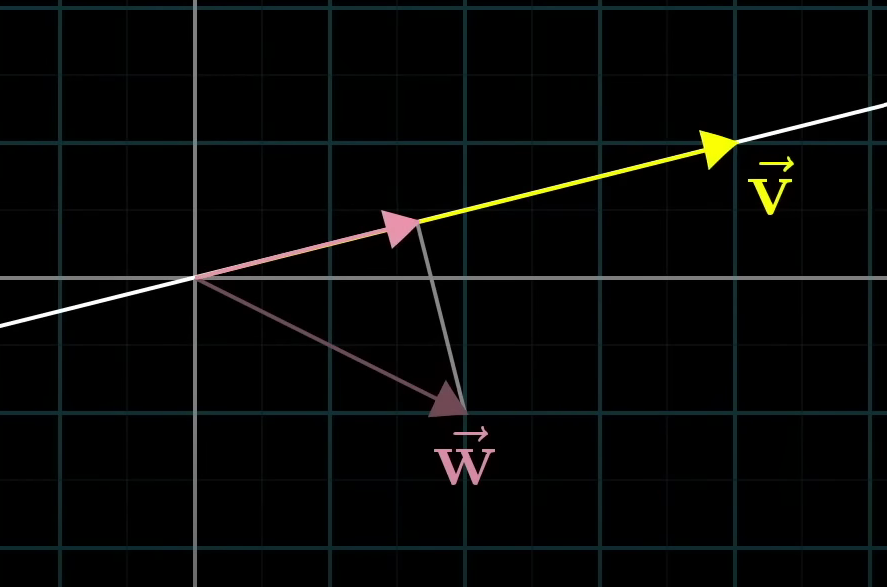
\includegraphics[scale=0.5]{dot product explination}
	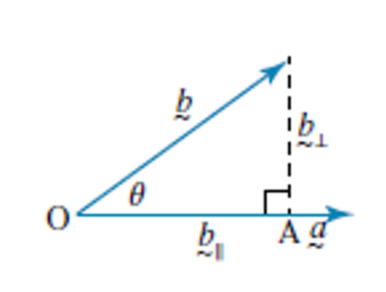
\includegraphics[scale=0.5]{dot product explination 2}
\end{center}
This can be calculated using the formula:
$$
	\Vec{OA} = |\utilde{b}|\cos\theta
$$
Where $\Vec{OA}$ is the line between the origin and the tip of the projected vector, $\utilde{b}$ is the vector being projected, and $\theta$ is the angle between the two vectors.  Or:
$$
	\Vec{OA} = \frac{\utilde{a} \cdot \utilde{b}}{|\utilde{a}|}
$$
And also:
$$
	\Vec{OA} = \hat{\utilde{a}} \cdot \utilde{b}
$$

\subsection{Vector resolutes}
The vector resolute is the same concept as the scalar resolute, but only that that we are concerned with the vector instead of the magnitude of the vector.  As we are projecting a vector onto another vector, we can simply multiply the result of the scalar resolute with the unit vector of the vector we are projecting onto:
$$
	\utilde{b}_{\parallel} = (\hat{\utilde{a}} \cdot \utilde{b}) \hat{\utilde{a}}
$$

Additionally, the vector perpendicular to the vector being projected to is given by:
$$
	\utilde{b}_{\perp} = \utilde{b} - (\hat{\utilde{a}} \cdot \utilde{b}) \hat{\utilde{a}}
$$

\subsection{Applications of vectors}
\subsubsection{Displacement and velocity}

\subsubsection{Triangle of forces}
% Resultant force

\subsection{Relative vectors}


\section{Proofs}
\subsection{Propositions}

\subsection{Direcct proofs}

\subsection{Proof by contraposition}
Proof by contraposition is done by proving the contrapositive

\subsection{Proof by contradiction}
Proof by contradiction is done by assuming that it is false initially.
\begin{enumerate}
	\item Assume (incorrectly) that what we want to prove is true, is actually false
	\item Show that the assumption eventually leads to mathematical nonsense
	\item Conclude that we are wrong to assume it is false
	\item realize that if it is not false, then it must be true
\end{enumerate}
Example:\\
$x$ satisfies $5^x = 2$, show that $x$ is irrational.++++
\begin{enumerate}
	\item Assume that $x$ is rational.
	\item $x = \frac{p}{q}, \in \int (\text{with no common factors})$ as all rational numbers can be represented by a fraction of integers
	\item $5^{\frac{p}{q}} = 2$
	\item $(5^{\frac{p}{q}})^q = (2)^q$
	\item $5^p = 2^p$
	\item odd = even
	\item $\therefore$ Contradiction, assumption was wrong.
	\item $\therefore$ $x$ is irrational.
\end{enumerate}

\section{Circles}
\subsection{Terms}

\subsection{Theorems}
\begin{center}
	\begin{tabular}[center]{p{5cm}|p{3cm}|p{2cm}}
		Theorem                                                                                                              & Diagram                                       & Symbol                                               \\ \hline
		The angle at the centre of the circle is twice the angle at the circumference subtended on the same arc.             & 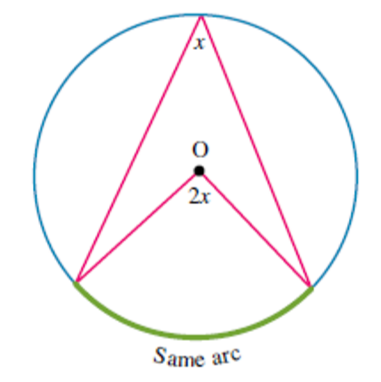
\includegraphics[width=3cm]{circle theorem 1} & 
\includegraphics[width=2cm]{circle theorem 1 symbol} \\
		Angles at the circumference subtended by the same arc are congruent.                                                 & 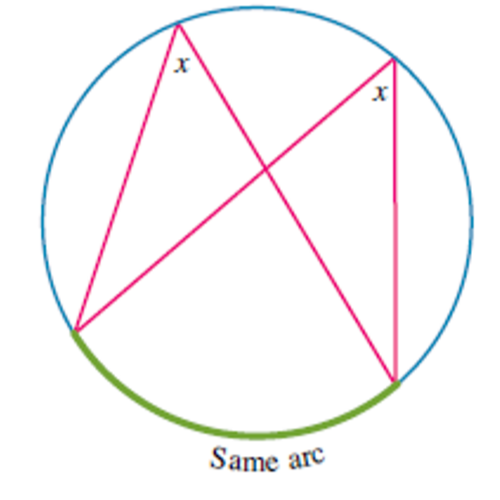
\includegraphics[width=3cm]{circle theorem 2} & 
\includegraphics[width=2cm]{circle theorem 2 symbol} \\
		The angle in a semicircle is a right angle.                                                                          & 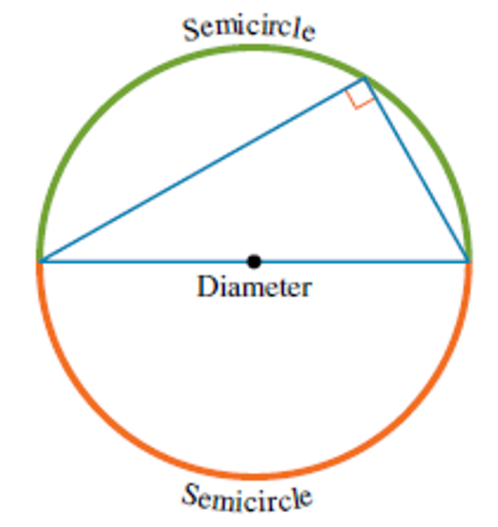
\includegraphics[width=3cm]{circle theorem 3} & 
\includegraphics[width=2cm]{circle theorem 3 symbol} \\
		If a line from the center bisects a chord, it is perpendicular to the chord.  The converse implication is also true. & 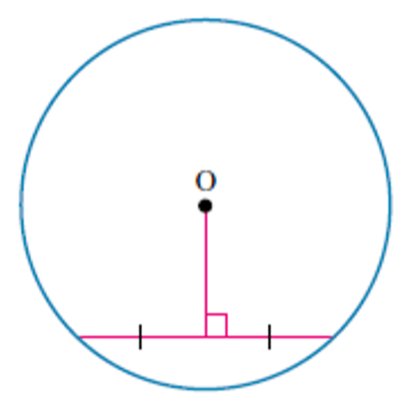
\includegraphics[width=3cm]{circle theorem 4} & 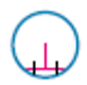
\includegraphics[width=2cm]{circle theorem 4 symbol} \\
		If the chords are congruent, then they are equidistant from the centre of the center.                                & 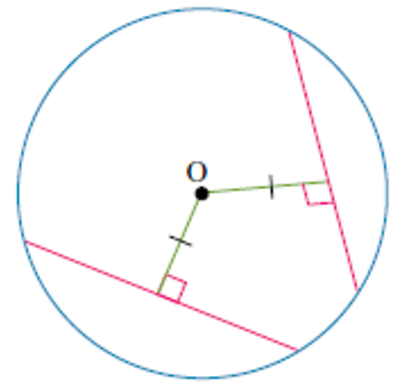
\includegraphics[width=3cm]{circle theorem 5} & 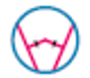
\includegraphics[width=2cm]{circle theorem 5 symbol} \\
	\end{tabular}
	\begin{tabular}[center]{p{5cm}|p{3cm}|p{2cm}}
		Theorem                                                                                                                                                                                        & Diagram                                        & Symbol                                                \\ \hline
		If two chords intersect inside the circle, then the point of intersection divides each chord into two segments so that the product of the lengths of the segments for both chords is the same. & 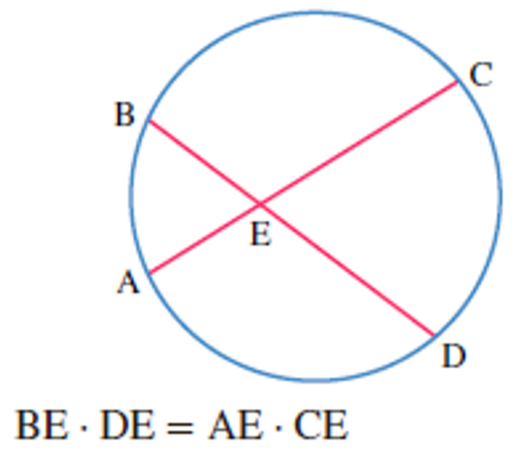
\includegraphics[width=3cm]{circle theorem 6}  & 
\includegraphics[width=2cm]{circle theorem 6 symbol}  \\
		If chords are congruent, they subtend equal angles at the centre.                                                                                                                              & 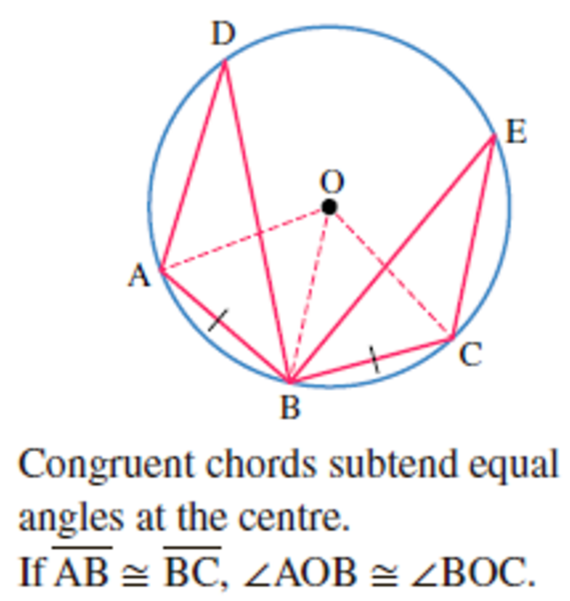
\includegraphics[width=3cm]{circle theorem 7}  & 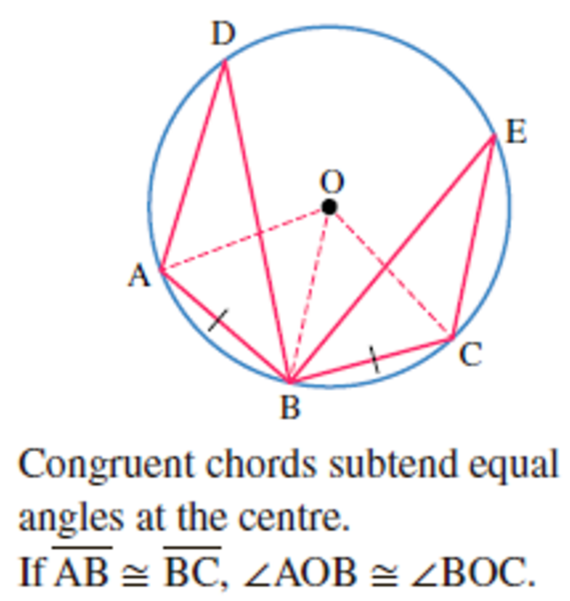
\includegraphics[width=2cm]{circle theorem 7 symbol}  \\
		A tangent and a radius intersects at right angles.                                                                                                                                             & 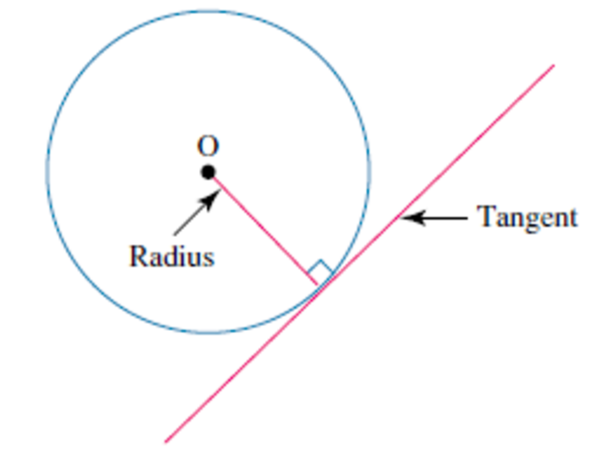
\includegraphics[width=3cm]{circle theorem 8}  & 
\includegraphics[width=2cm]{circle theorem 8 symbol}  \\
		Two tangents drawn from an external point to a circle are congruent.                                                                                                                           & 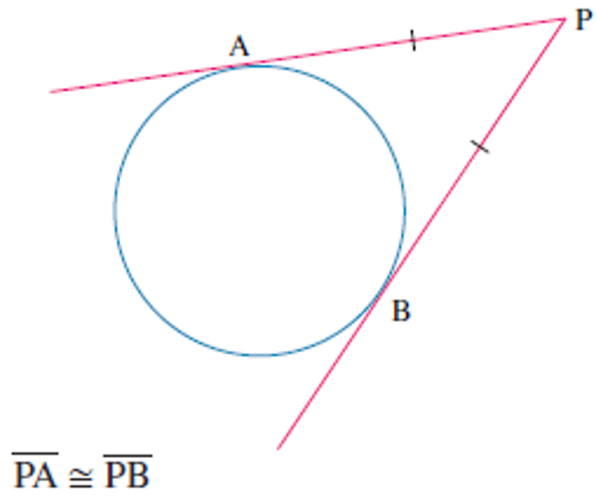
\includegraphics[width=3cm]{circle theorem 9}  & 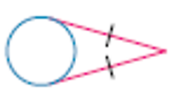
\includegraphics[width=2cm]{circle theorem 9 symbol}  \\
		The angle formed by two tangents meeting at an external point is bisected by a straight line joining the centre of the circle to that external point.                                          & 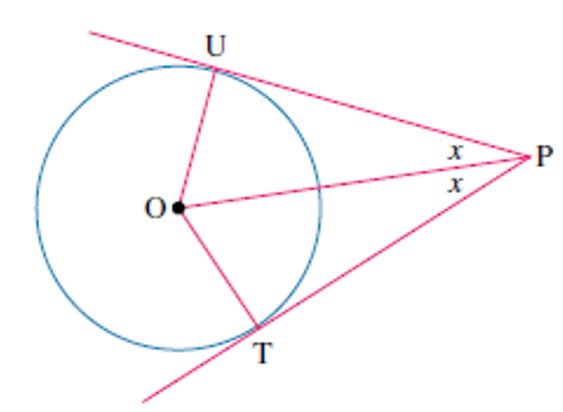
\includegraphics[width=3cm]{circle theorem 10} & 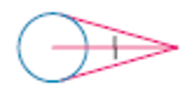
\includegraphics[width=2cm]{circle theorem 10 symbol} \\
	\end{tabular}
	\begin{tabular}[center]{p{5cm}|p{3cm}|p{2cm}}
		Theorem                                                                                                                                                                                                                      & Diagram                                        & Symbol                                                \\ \hline
		The angle formed by a tangent and a chord is congruent to the angle in the alternate segment.                                                                                                                                & 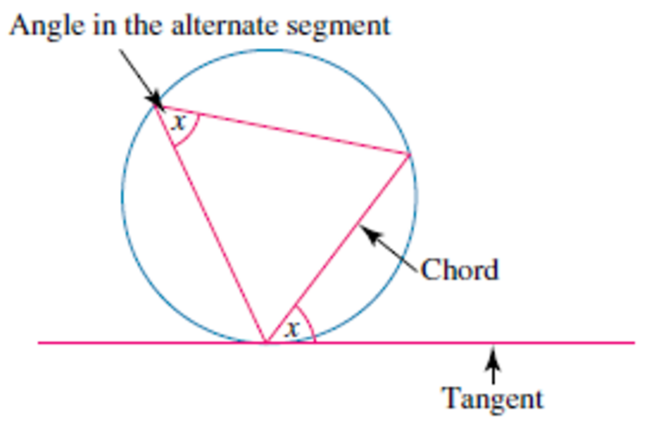
\includegraphics[width=3cm]{circle theorem 11} & 
\includegraphics[width=2cm]{circle theorem 11 symbol} \\
		If a secant (meeting the circle at A and B) and a tangent (meeting at circle at T) are drawn from an external point P, the square of the length of the tangent equals the product of the length to the circle on the secant. & 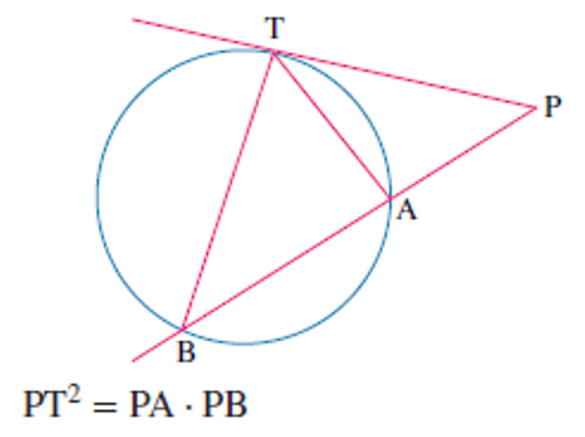
\includegraphics[width=3cm]{circle theorem 12} & 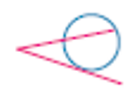
\includegraphics[width=2cm]{circle theorem 12 symbol} \\
		If two secants intersect outside the circle, then the product of one external secant segment length and it's external length is equal to the product of the other secant lengths.                                            & 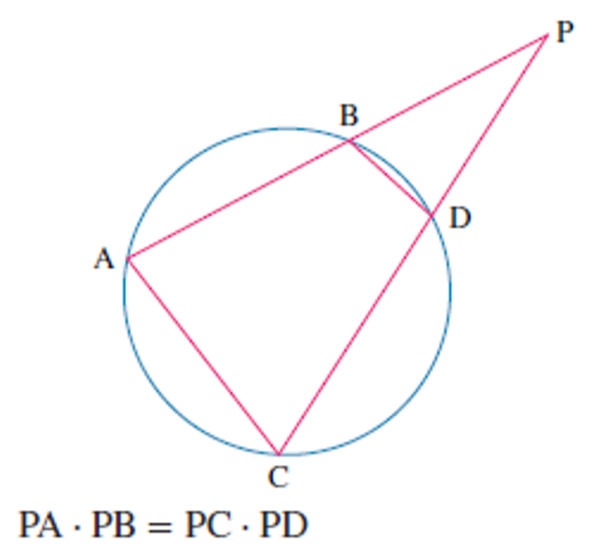
\includegraphics[width=3cm]{circle theorem 13} & 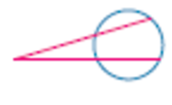
\includegraphics[width=2cm]{circle theorem 13 symbol} \\
		The opposite angles of a cyclic quadrilateral are supplementary.                                                                                                                                                             & 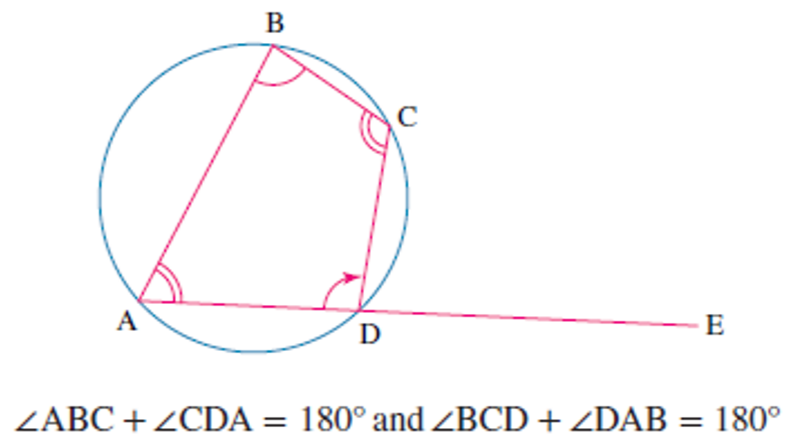
\includegraphics[width=3cm]{circle theorem 14} & 
\includegraphics[width=2cm]{circle theorem 14 symbol} \\
		The exterior angle of a cyclic quadrilateral is congruent to the inner opposite angle.                                                                                                                                       & 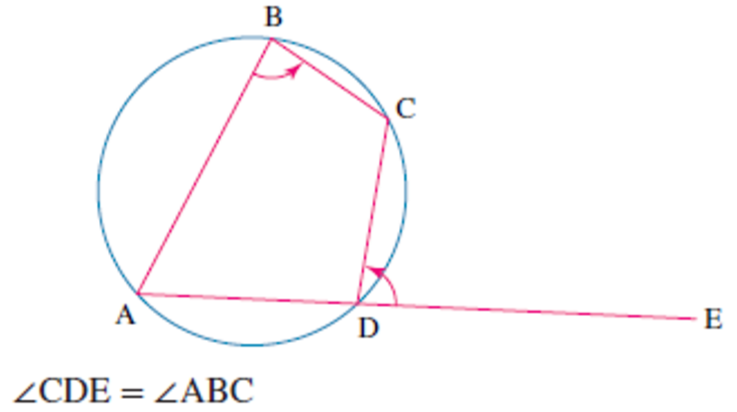
\includegraphics[width=3cm]{circle theorem 15} & 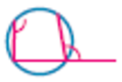
\includegraphics[width=2cm]{circle theorem 15 symbol}
	\end{tabular}
\end{center}


\end{document}